The objective of the project is to collect as much information as possible about the performance of the production process, with a focus on both dough balls and final baked bread.\\
To determine the position of loaves and dough units at different stages of the process, a real-time deep learning network based on \textbf{DETR (DEtection TRansformer)} is employed for object detection.\\
Once the bounding boxes have been identified, downstream analysis is performed differently at the two acquisition sites. \\
At Site 1, the \textbf{volume} of each dough ball is estimated from RGB-D data.\\
At Site 2, instead of directly extracting handcrafted color and shape descriptors, a dedicated \textbf{anomaly detection network} is applied to the loaf regions to identify potentially defective products.\\
To achieve this, the system is deployed across two acquisition sites:
\begin{itemize}
    \item \textbf{Site 1}: located at the output of the dough processing stage.\\
    At this site, a \textbf{NVIDIA Jetson Nano} is connected to a \textbf{Microsoft Azure Kinect} sensor, which is installed to acquire RGB-D data. These data are subsequently processed to estimate the dough volume.
    \item \textbf{Site 2}: located at the point where bread is removed from the baking tray.\\
    At this site, a \textbf{Raspberry Pi 5} equipped with a \textbf{Raspberry Pi Camera} captures RGB images of the loaves. These images are analyzed by an anomaly detection model to flag non-conforming products.
\end{itemize}

\begin{figure}[h]
    \centering
    \begin{subfigure}[t]{0.48\textwidth}
        \centering
        \vspace{0pt}% allinea in alto
        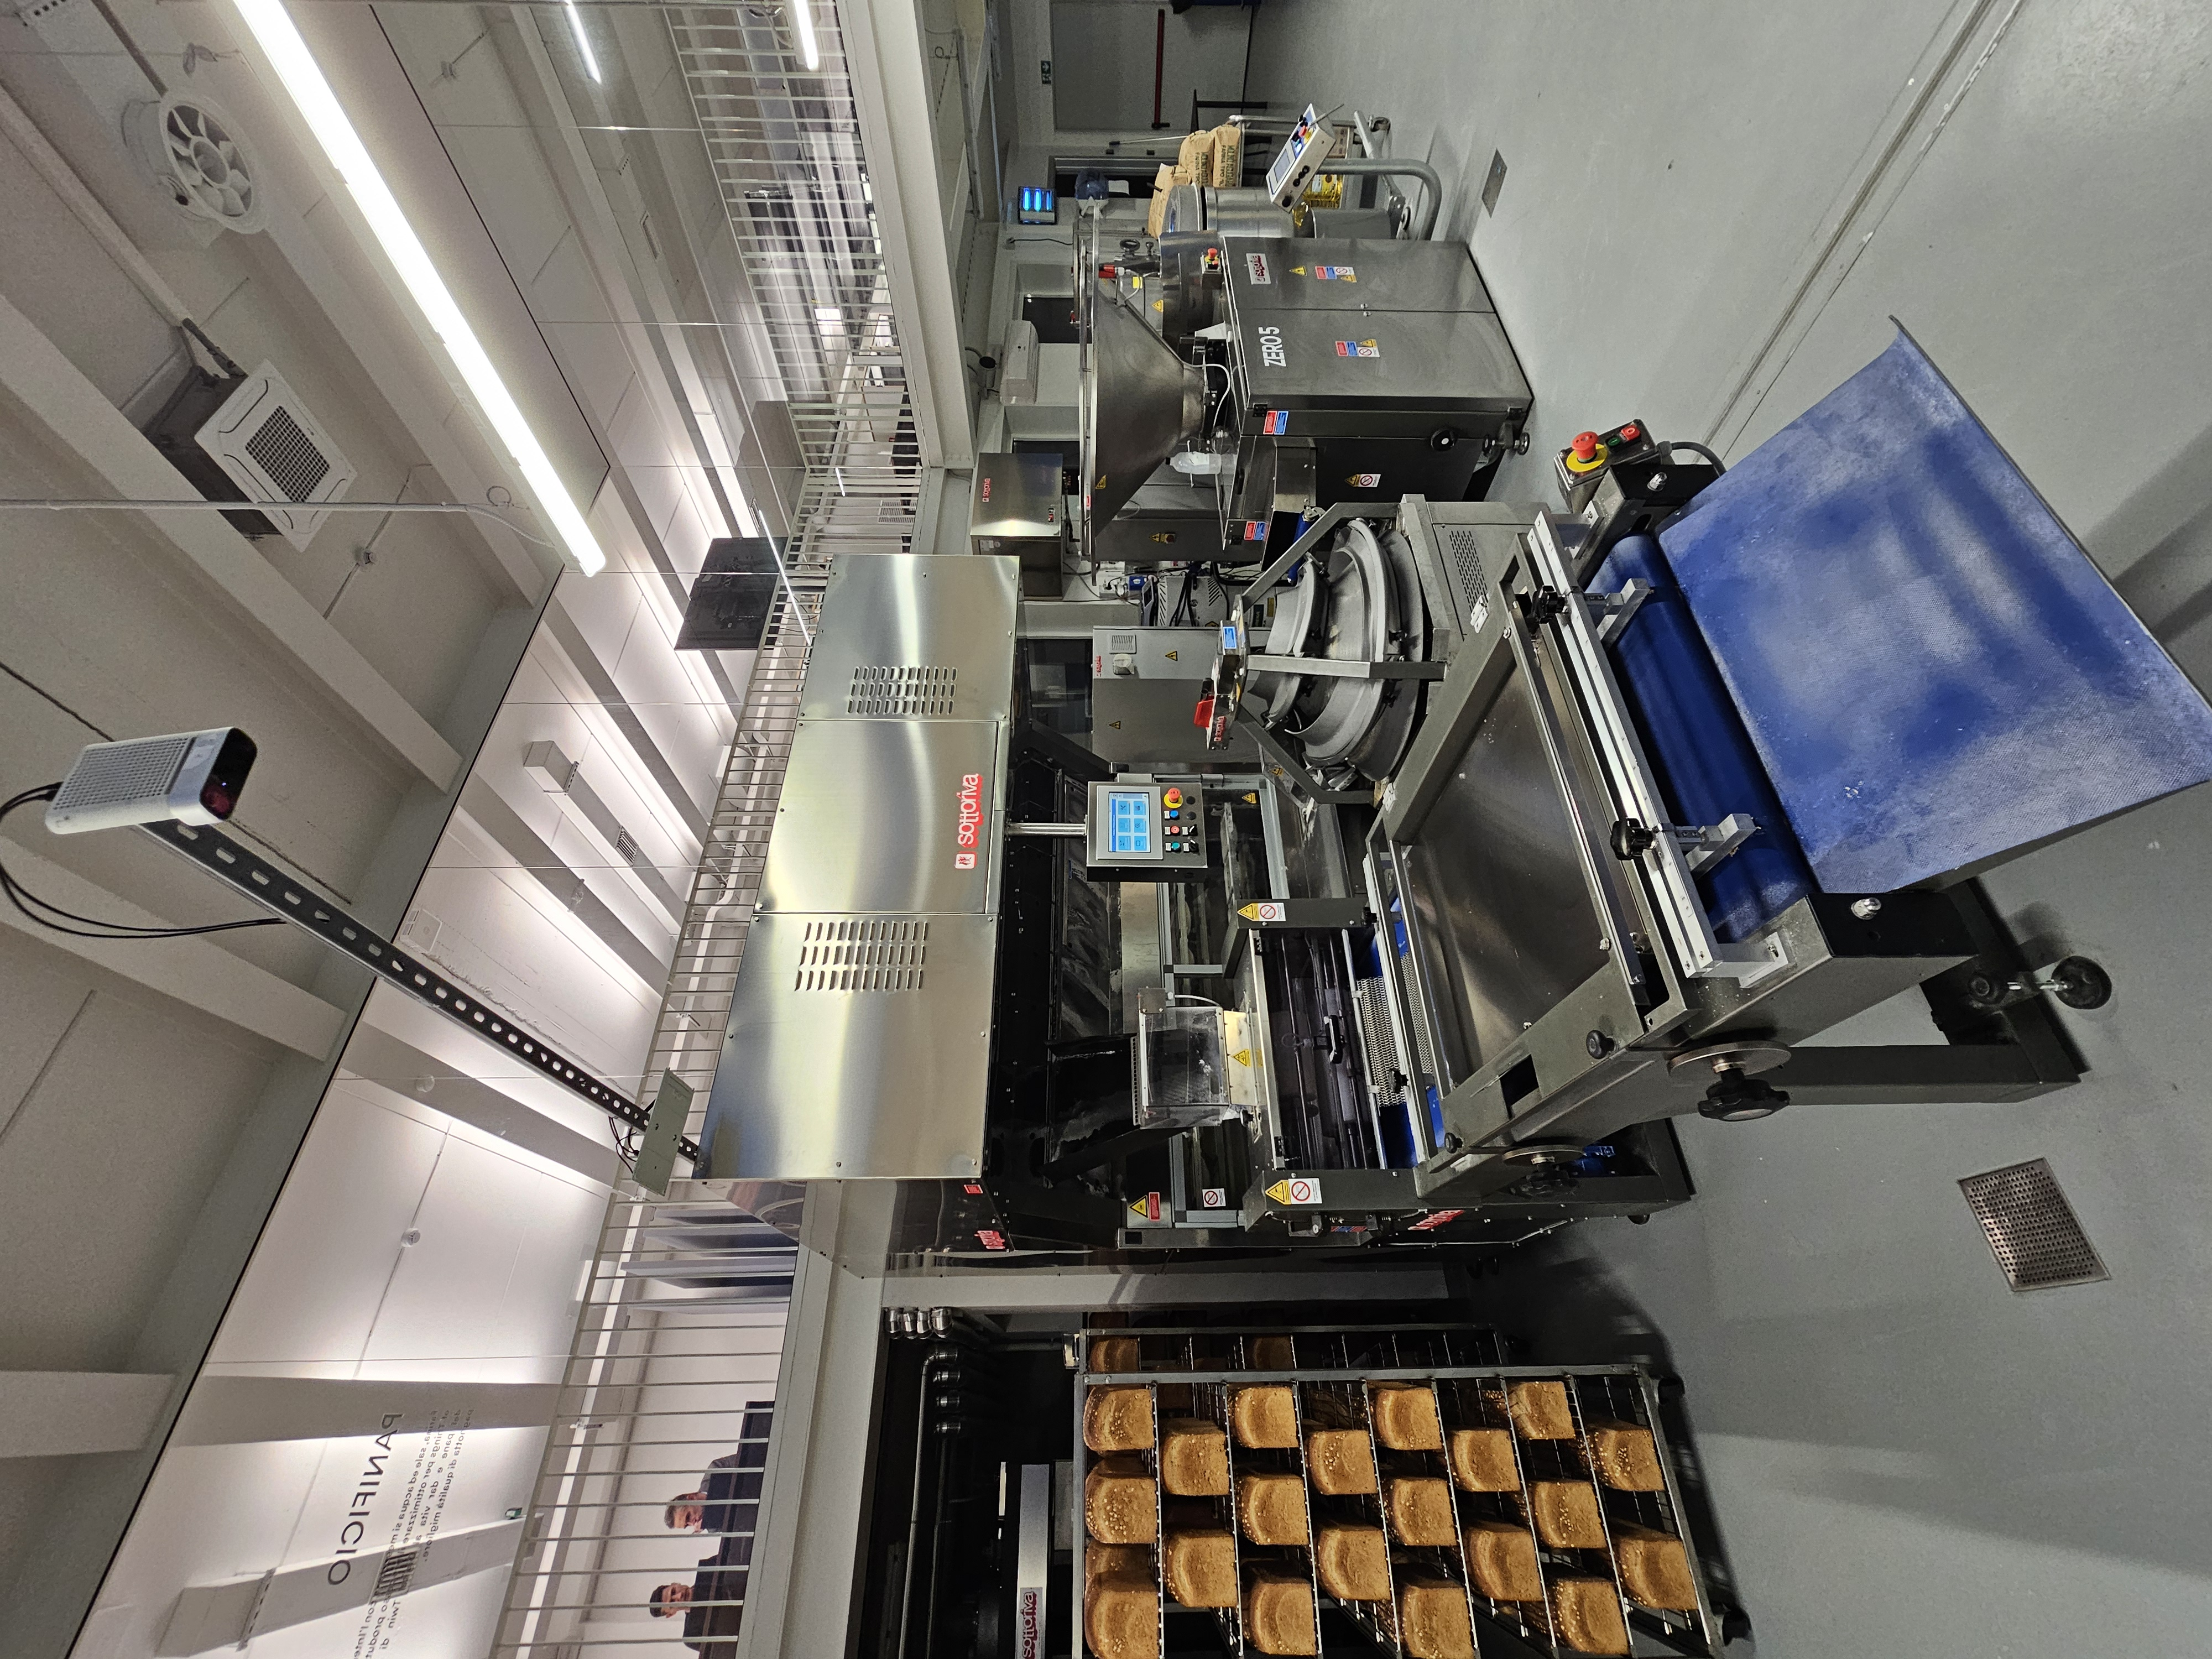
\includegraphics[scale=0.07, angle=-90]{images/Site1.jpg}
        \caption{Site 1: from here the dough balls come out and stop on the blue tray}
        \label{fig:site1}
    \end{subfigure}\hfill
    \begin{subfigure}[t]{0.48\textwidth}
        \centering
        \vspace{0pt}% allinea in alto
        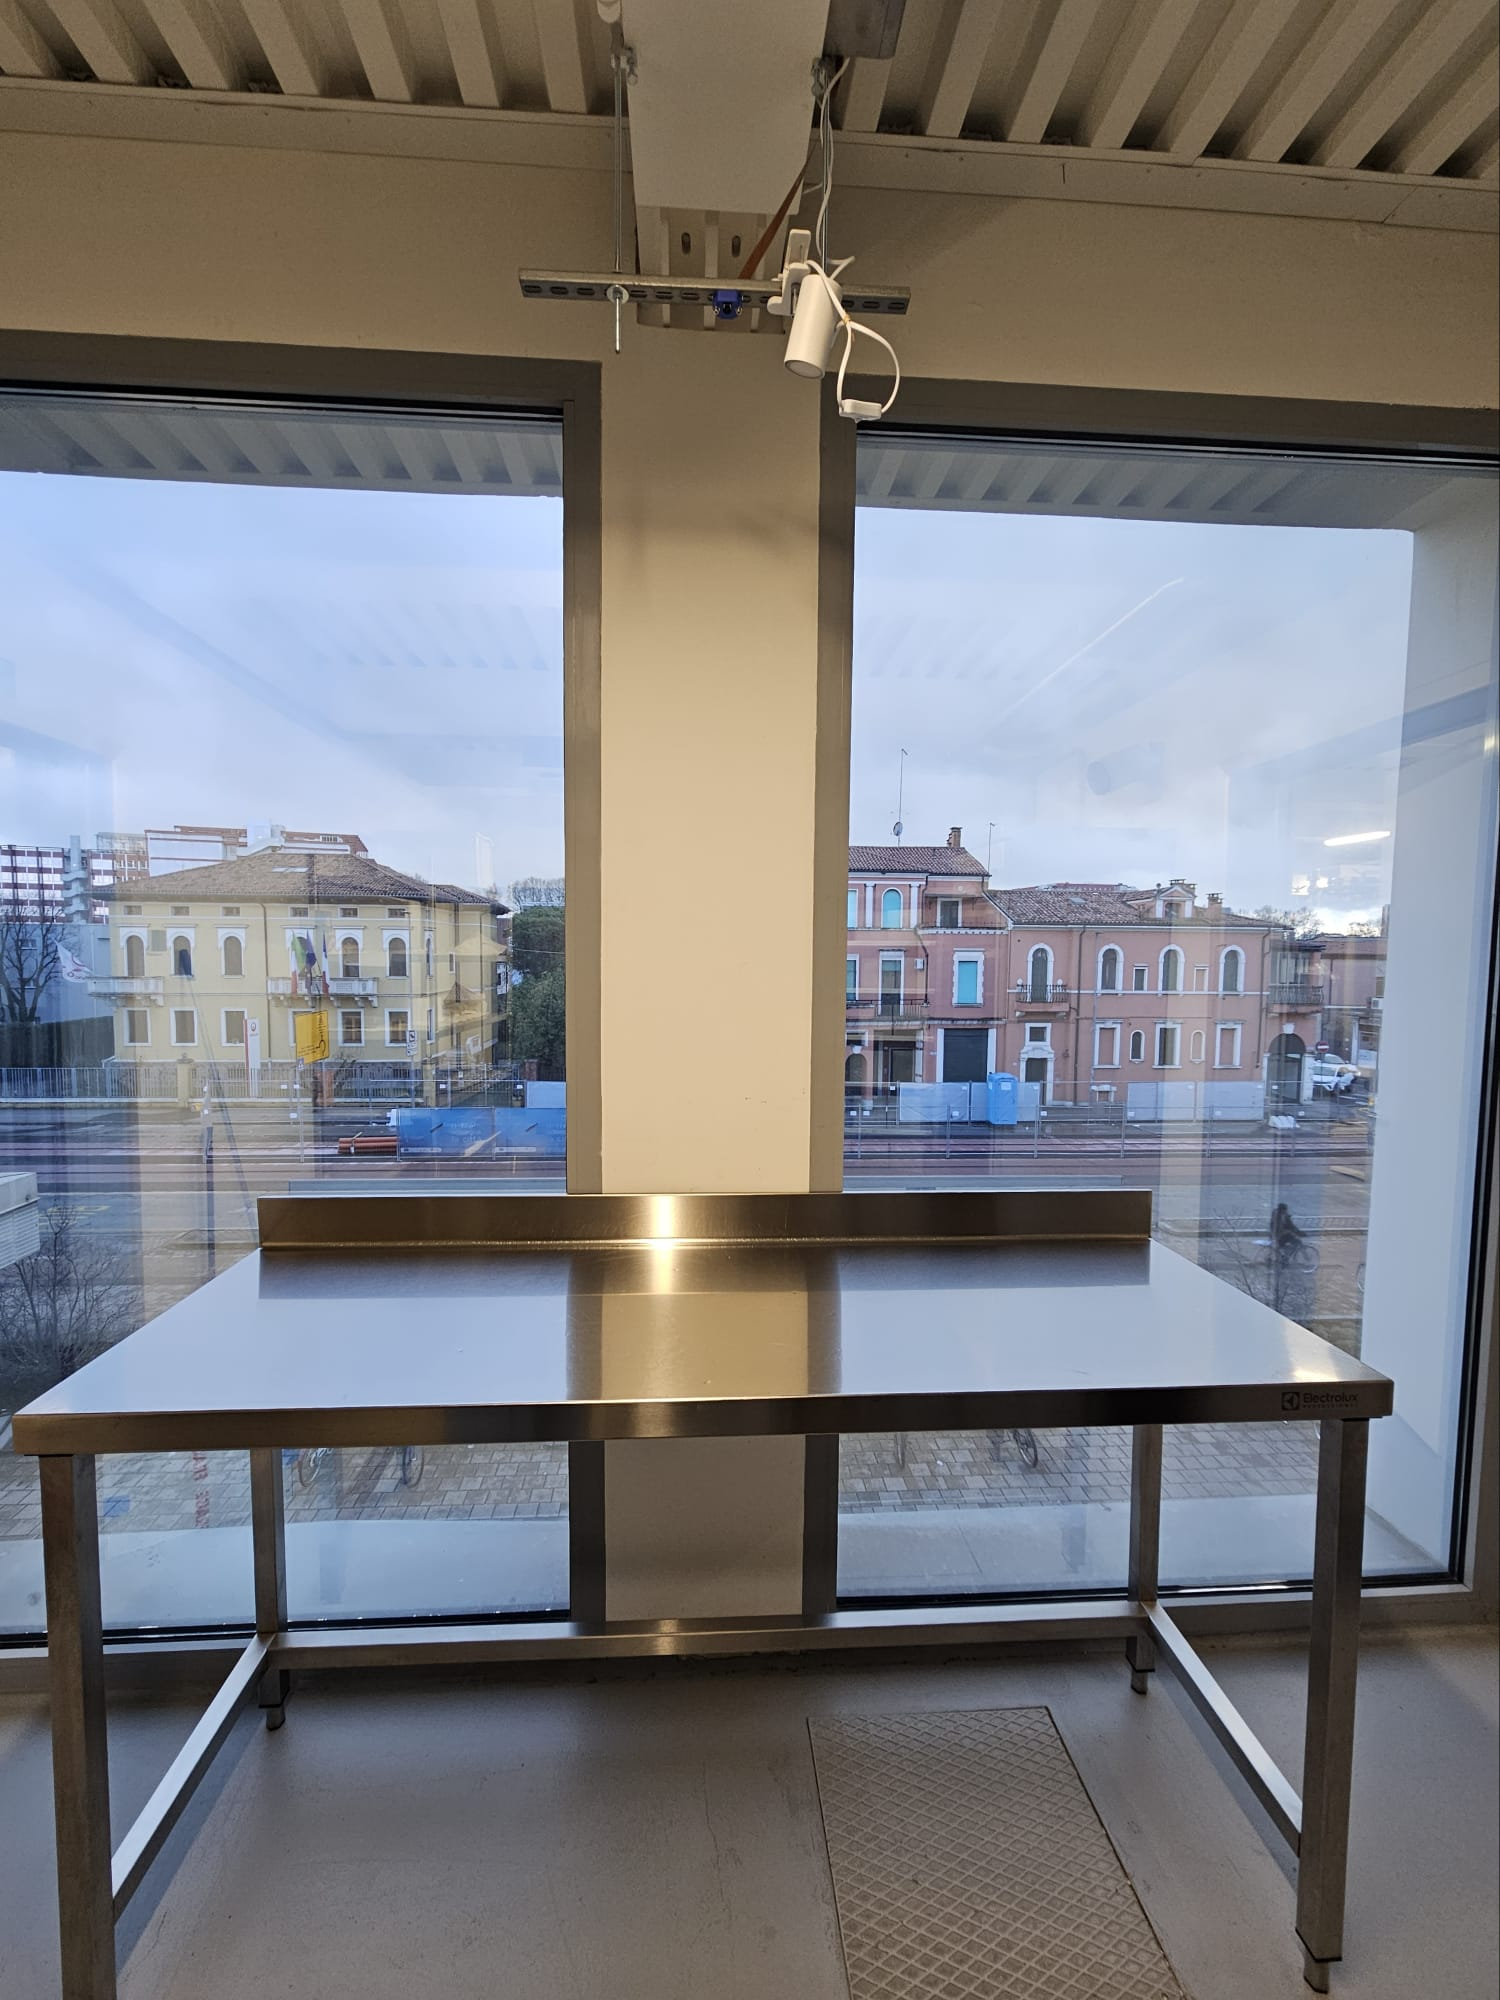
\includegraphics[scale=0.14]{images/sito2_giorno.jpeg}
        \caption{Site 2: area where bread is baked}
        \label{fig:site2}
    \end{subfigure}
    \caption{Overview of Site 1 and Site 2}
    \label{fig:sites12}
\end{figure}

Ultimately, once all the data have been extracted and processed, statistical distributions of dough ball volumes and anomaly scores for baked loaves are constructed. These distributions constitute the final analytical output of the system and provide a quantitative overview of production performance.

For each monitored variable, descriptive statistical indicators such as mean value, variance, and standard deviation are computed. The mean provides an estimate of the nominal production target, while the variance and standard deviation quantify dispersion and process variability. 

By analyzing both the distribution curves and their associated statistical descriptors, it becomes possible to evaluate the consistency and repeatability of the production process across different time intervals. In particular, deviations in volume distributions may indicate instability in the forming stage, whereas systematic shifts in anomaly-score distributions may reveal variations in baking conditions or product quality.
\newline

The resulting statistical summary therefore represents a quantitative decision-support tool for quality assessment. Rather than relying solely on qualitative visual inspection, the proposed framework enables objective measurement of process stability, variability, and deviation from expected operating conditions.

In this context, the thesis demonstrates how computer vision and embedded AI systems can be integrated into an industrial environment to transform raw sensory data into actionable statistical insights, bridging the gap between low-level image acquisition and high-level production performance evaluation. 

